\documentclass[stu,12pt,floatsintext]{apa7}
\usepackage[american]{babel}
\usepackage{csquotes} 
\usepackage[style=apa,sortcites=true,sorting=nyt,backend=biber]{biblatex}
\DeclareLanguageMapping{american}{american-apa}
\addbibresource{bibliography.bib} 

\usepackage[T1]{fontenc} 
\usepackage{mathptmx} 


\title{Designing a Data Platform Prototype for UAV Hyperspectral Crop Trait Retrieval Model Development and Evaluation at Agroscope} 
\shorttitle{Phenobase} 
\author{Pascal Ackermann}
\duedate{December 18, 2026}
\authorsaffiliations{Hochschule Luzern HSLU}
\course{Master Thesis} 
\professor{Oliver Staubli, Dr. Francesco Argento, Dr. Helge Aasen}  

\abstract{Insert abstract text here.}
\keywords{UAV, Croptrait, Hyperspectral} 

\begin{document}


\maketitle 

Biophysical crop traits such as above-ground biomass, plant height, and leaf area index are fundamental indicators of plant health, growth status, and yield potential \parencite{li_review_2026}. Monitoring these traits throughout the growing season enables early detection of stress, assessment of fertilization efficiency, and estimation of expected yields, information that is directly relevant for agricultural research, regional food security planning, and evidence-based policy making. Traditionally assessing biophysical crop traits relies on in-situ measurements collected through destructive or non-destructive sampling methods, which are labor-intensive, time-consuming, and spatially limited in their coverage \parencite{kumar_remote_2017}.

Unmanned Aerial Vehicles (UAVs) equipped with hyperspectral cameras offer a scalable alternative, capturing reflected light across hundreds of spectral bands that encode subtle biochemical and structural properties of vegetation invisible to conventional RGB cameras. Applying crop trait retrieval models to such hyperspectral UAV imagery enables the spatial prediction of key crop traits at field scale, at high resolution, and without physical contact with the plant. These properties have made UAV-based hyperspectral sensing an increasingly central tool in precision agriculture and plant phenotyping research \parencite{li_review_2026}

Crop traits can be retrieved from UAV imagery using different approaches, such as radiative transfer models (RTM), vegetation indices (VIs) and machine learning models.
RTMs are physics-based models that link crop traits to their spectral signatures. A widely used RTM is PROSAIL \parencite{bhadra_prosail-net_2024,noauthor_eoa-teamprosail_forward_2026, gomez-dans_jgomezdansprosail_2026, jacquemoud_prospect_2009}, which simulates canopy reflectance and stores the corresponding crop traits in a Look-Up Table (LUT). By running the model in inverse mode, users can retrieve specific crop traits by matching measured UAV reflectance against the simulated values in the LUT. VIs are calculated from specific spectral band combinations tied to known plant absorption features. Widely used examples include NDVI and  EVI \parencite{radocaj_state_2023}. These indices serve as spectral proxies for biophysical crop traits, providing interpretable and computationally lightweight estimates directly from reflectance data. Machine learning (ML) models, on the other hand, offer maximum flexibility in their input features; they can make use of raw spectral bands, precomputed VIs, retrieved crop traits  or a combination of all three. This allows them to capture complex, non-linear relationships, that VIs fail to resolve 

While VIs are widely used for their simplicity and reliability, machine learning models are attracting growing interest due to their potential to outperform traditional indices. This is particularly true when models are applied across diverse crop types, varying environmental conditions, or to estimate traits with no well-established spectral proxy. \parencite{kumar_remote_2017}). 




\section{Introduction}

Lorem ipsum dolor sit amet, consetetur sadipscing elitr, sed diam nonumy eirmod tempor invidunt ut labore et dolore magna aliquyam erat, sed diam voluptua. At vero eos et accusam et justo duo dolores et ea rebum. Stet clita kasd gubergren, no sea takimata sanctus est Lorem ipsum dolor sit amet. Lorem ipsum dolor sit amet, consetetur sadipscing elitr, sed diam nonumy eirmod tempor invidunt ut labore et dolore magna aliquyam erat, sed diam voluptua. At vero eos et accusam et justo duo dolores et ea rebum. Stet clita kasd gubergren, no sea takimata sanctus est Lorem ipsum dolor sit amet.

\subsection{Potential of of UAV-based hyperspectral sensing for plant phenotyping research}

Lorem ipsum dolor sit amet, consetetur sadipscing elitr, sed diam nonumy eirmod tempor invidunt ut labore et dolore magna aliquyam erat, sed diam voluptua. At vero eos et accusam et justo duo dolores et ea rebum. Stet clita kasd gubergren, no sea takimata sanctus est Lorem ipsum dolor sit amet. Lorem ipsum dolor sit amet, consetetur sadipscing elitr, sed diam nonumy eirmod tempor invidunt ut labore et dolore magna aliquyam erat, sed diam voluptua. At vero eos et accusam et justo duo dolores et ea rebum. Stet clita kasd gubergren, no sea takimata sanctus est Lorem ipsum dolor sit amet.

\section{Literature Review}

Lorem ipsum dolor sit amet, consetetur sadipscing elitr, sed diam nonumy eirmod tempor invidunt ut labore et dolore magna aliquyam erat, sed diam voluptua. At vero eos et accusam et justo duo dolores et ea rebum. Stet clita kasd gubergren, no sea takimata sanctus est Lorem ipsum dolor sit amet. Lorem ipsum dolor sit amet, consetetur sadipscing elitr, sed diam nonumy eirmod tempor invidunt ut labore et dolore magna aliquyam erat, sed diam voluptua. At vero eos et accusam et justo duo dolores et ea rebum. Stet clita kasd gubergren, no sea takimata sanctus est Lorem ipsum dolor sit amet.

\section{Exploration}

\section{Requirements Engineering }

\subsection{Participants}

Participant information goes here.

\subsection{Materials}

Words, along with a sample table (Table~\ref{tab:table_words}).

% There's lots of little components to the table. For the most part you can just copy it, or build your own with Overleaf's table wizard up top. 
% I'll mention that the & character separates items into different columns on a row, and the \\ ends that line. \hline generates a line that matches the width of the table.
\begin{table}
    \caption{Sample words from this hypothetical experiment.}
    \centering
    \begin{tabular}{cc} %The c's here indicate the columns will be centered
        \hline 
         First word & Second word \\
         \hline
         Yeet & Yoink \\
         Hot & Lit \\
         \hline
    \end{tabular}
    \label{tab:table_words}
\end{table}


\subsection{Measures}

Some words about the measures used.

\subsection{Design}

Some more words


\subsection{Procedure}

Description of the procedure.



\section{Results}

\subsection{Descriptive Statistics}

Statistical words. A demonstrative Figure~\ref{fig:OverallEffect}.

\begin{figure}
    \centering
    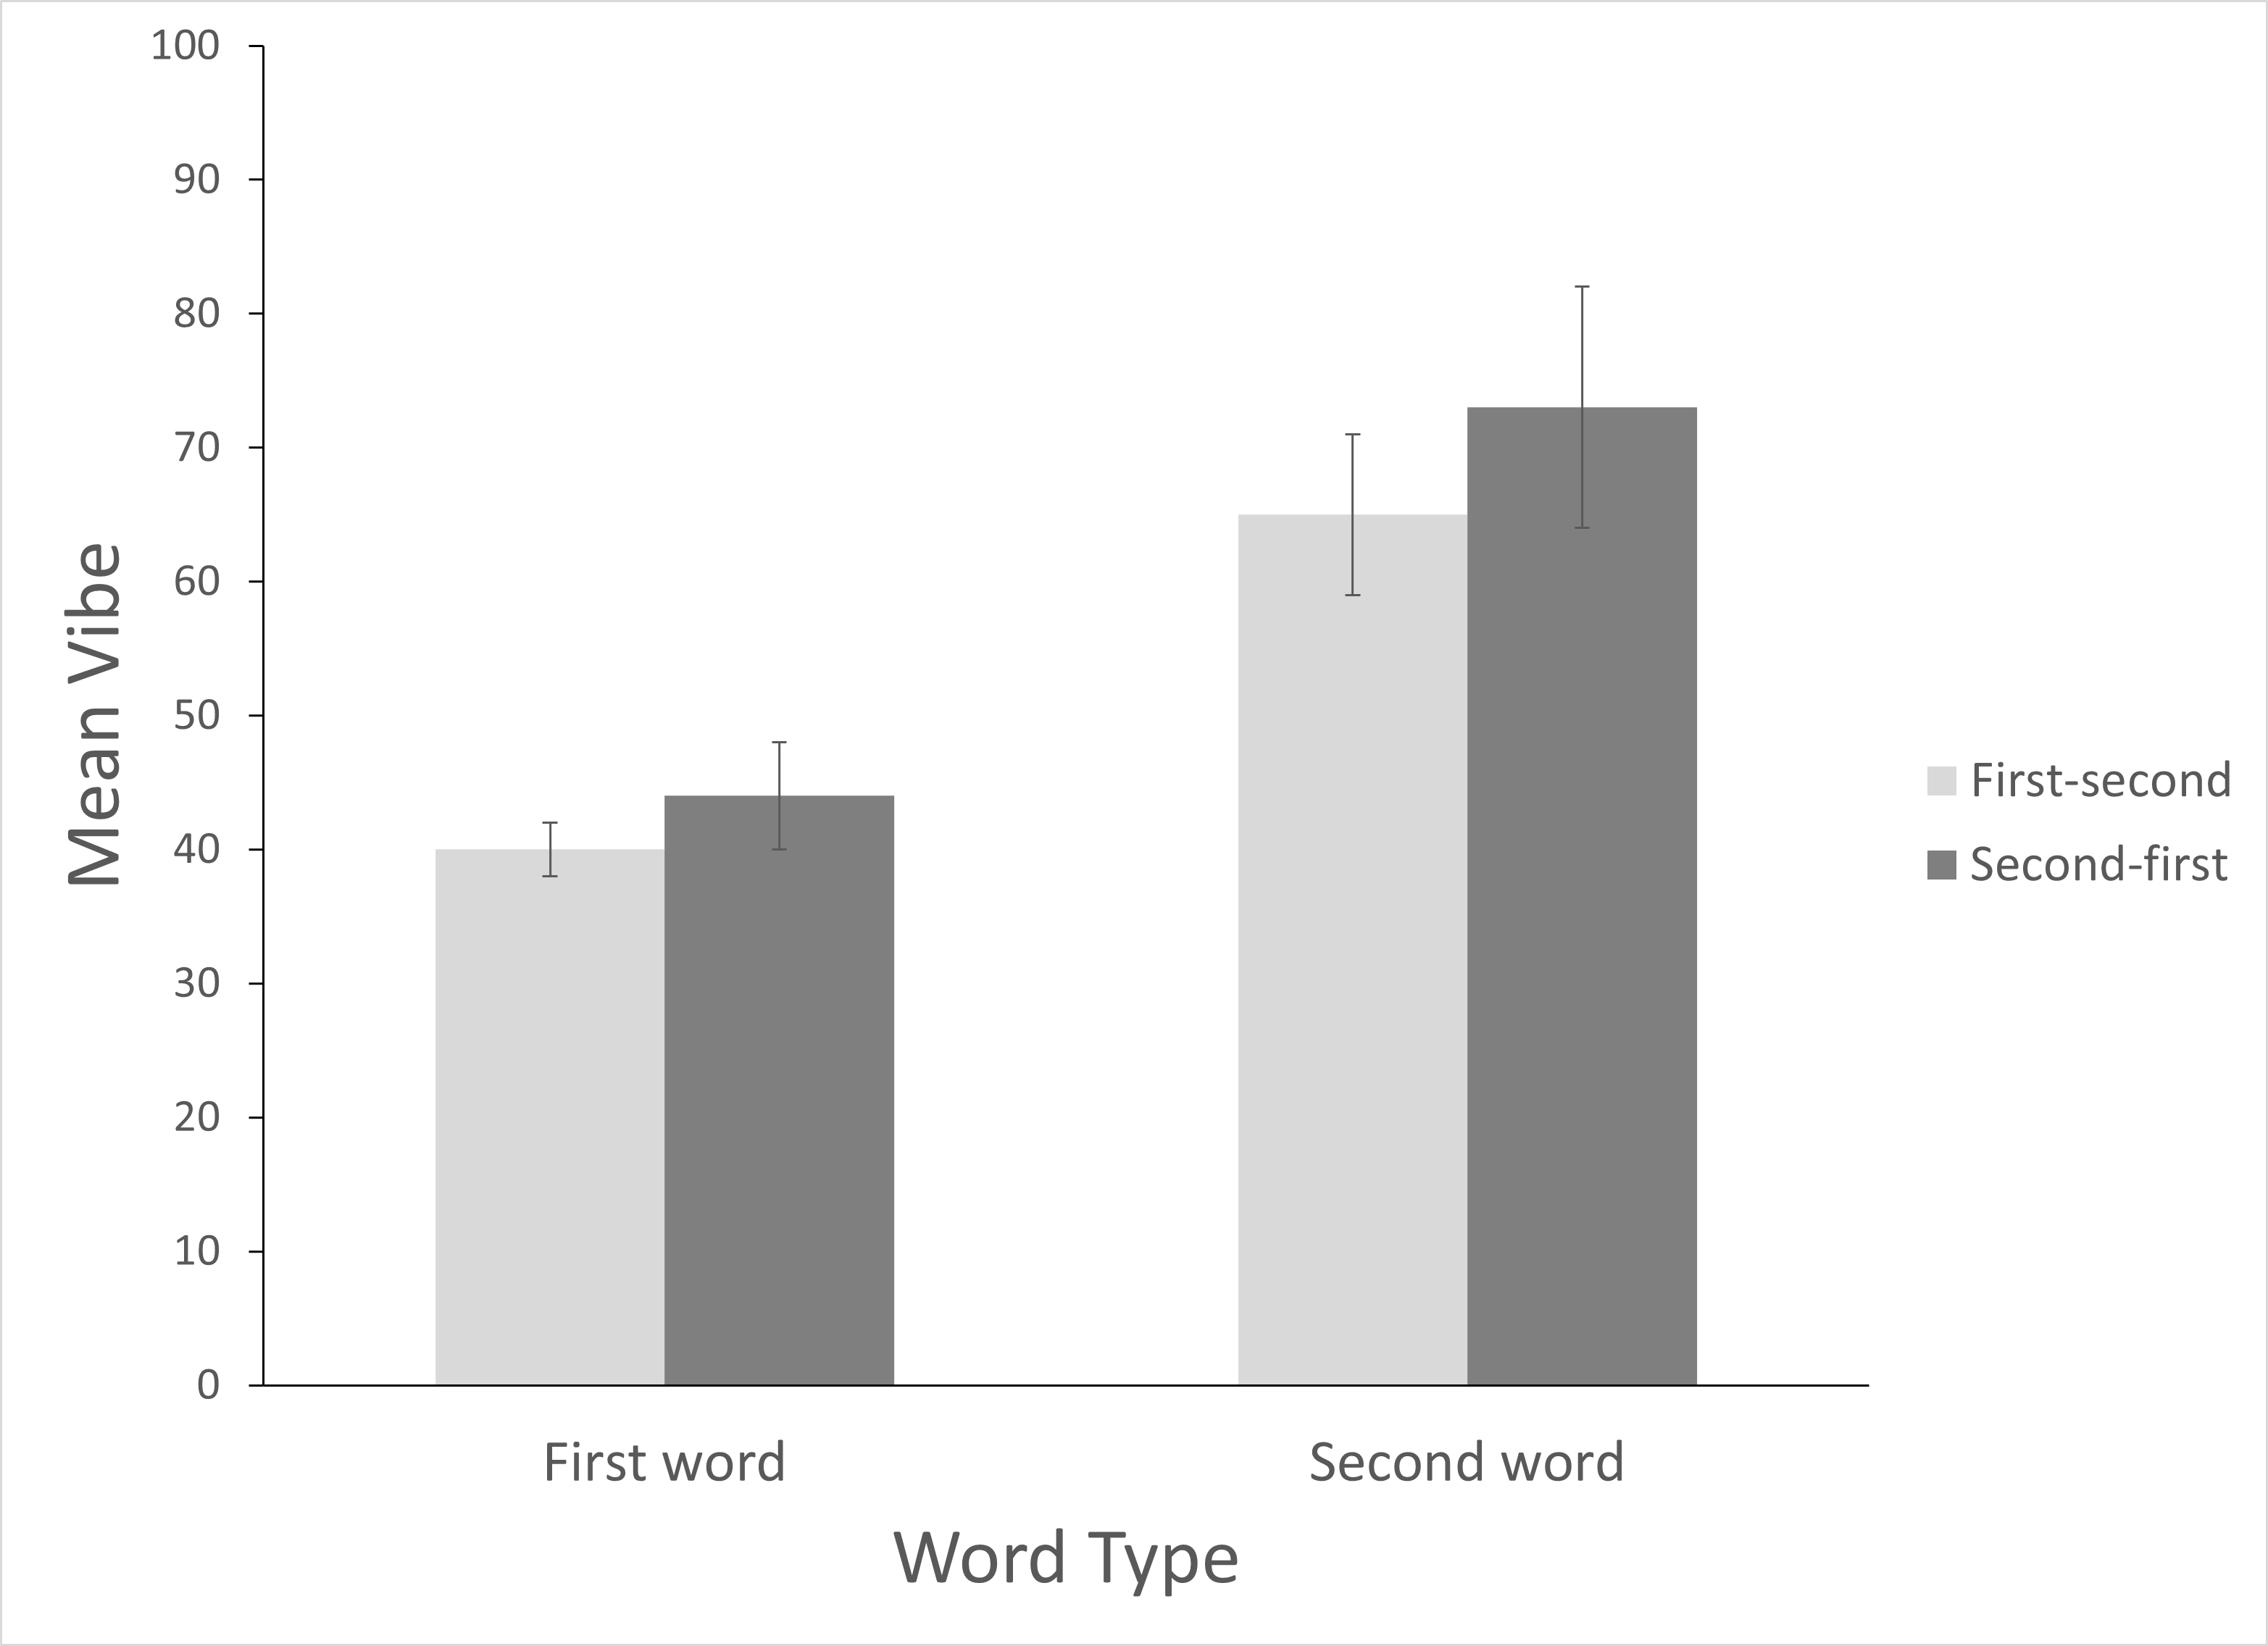
\includegraphics[width=0.75\linewidth]{sampleFig.png} % This is setting the figure to be .75x the width of the line. This can go all the way from 0.1 to 1 (and beyond, but then you're outside the page).
    \caption{The mean vibes for each word type and counterbalanced condition order. Error bars represent one standard error of the mean.}
    \label{fig:OverallEffect}
\end{figure}

\subsection{Inferential Statistics}

Analytical words.

\section{Discussion}

Discussion words.



\printbibliography

\end{document}

%% 
%% Copyright (C) 2019 by Daniel A. Weiss <daniel.weiss.led at gmail.com>
%% 
%% This work may be distributed and/or modified under the
%% conditions of the LaTeX Project Public License (LPPL), either
%% version 1.3c of this license or (at your option) any later
%% version.  The latest version of this license is in the file:
%% 
%% http://www.latex-project.org/lppl.txt
%% 
%% Users may freely modify these files without permission, as long as the
%% copyright line and this statement are maintained intact.
%% 
%% This work is not endorsed by, affiliated with, or probably even known
%% by, the American Psychological Association.
%% 
%% This work is "maintained" (as per LPPL maintenance status) by
%% Daniel A. Weiss.
%% 
%% This work consists of the file  apa7.dtx
%% and the derived files           apa7.ins,
%%                                 apa7.cls,
%%                                 apa7.pdf,
%%                                 README,
%%                                 APA7american.txt,
%%                                 APA7british.txt,
%%                                 APA7dutch.txt,
%%                                 APA7english.txt,
%%                                 APA7german.txt,
%%                                 APA7ngerman.txt,
%%                                 APA7greek.txt,
%%                                 APA7czech.txt,
%%                                 APA7turkish.txt,
%%                                 APA7endfloat.cfg,
%%                                 Figure1.pdf,
%%                                 shortsample.tex,
%%                                 longsample.tex, and
%%                                 bibliography.bib.
%% 
%%
%%
%% This is file `./samples/shortsample.tex',
%% generated with the docstrip utility.
%%
%% The original source files were:
%%
%% apa7.dtx  (with options: `shortsample')
%% ----------------------------------------------------------------------
%% 
%% apa7 - A LaTeX class for formatting documents in compliance with the
%% American Psychological Association's Publication Manual, 7th edition
%% 
%% Copyright (C) 2019 by Daniel A. Weiss <daniel.weiss.led at gmail.com>
%% 
%% This work may be distributed and/or modified under the
%% conditions of the LaTeX Project Public License (LPPL), either
%% version 1.3c of this license or (at your option) any later
%% version.  The latest version of this license is in the file:
%% 
%% http://www.latex-project.org/lppl.txt
%% 
%% Users may freely modify these files without permission, as long as the
%% copyright line and this statement are maintained intact.
%% 
%% This work is not endorsed by, affiliated with, or probably even known
%% by, the American Psychological Association.
%% 
%% ----------------------------------------------------------------------